\chaptr{Anexos}{anexos}
\sect{Anexo A: Pila del producto}{anexoA}

Durante el desarrollo del proyecto se han realizado una serie de tareas, para las cuales se ha utilizado la
herramienta \boldFont{Notion}.
Esta herramienta proporciona una interfaz muy sencilla para la creación de tareas, con la
posibilidad de añadir etiquetas, asignar responsables, añadir comentarios a cada una de ellas,
entre otras funcionalidades.
A continuación, se incluye el fichero pdf generado por Notion con la pila del producto completa.\ Además, se puede
consultar la pila del producto de una manera más interactiva en el siguiente enlace:
\href{https://scastd00.notion.site/9c59c2812d8b440faa453924fef2f320?v=20f7c2f47dd64574ac57713e8efe2718}
{https://scastd00.notion.site/9c59c2812d8b440faa453924fef2f3
20?v=20f7c2f47dd64574ac57713e8efe2718}

% Generar el pdf a 57% de tamaño para que quepa el ancho de página incluyendo las notas de Notion.
\label{anx:product-backlog-notion}
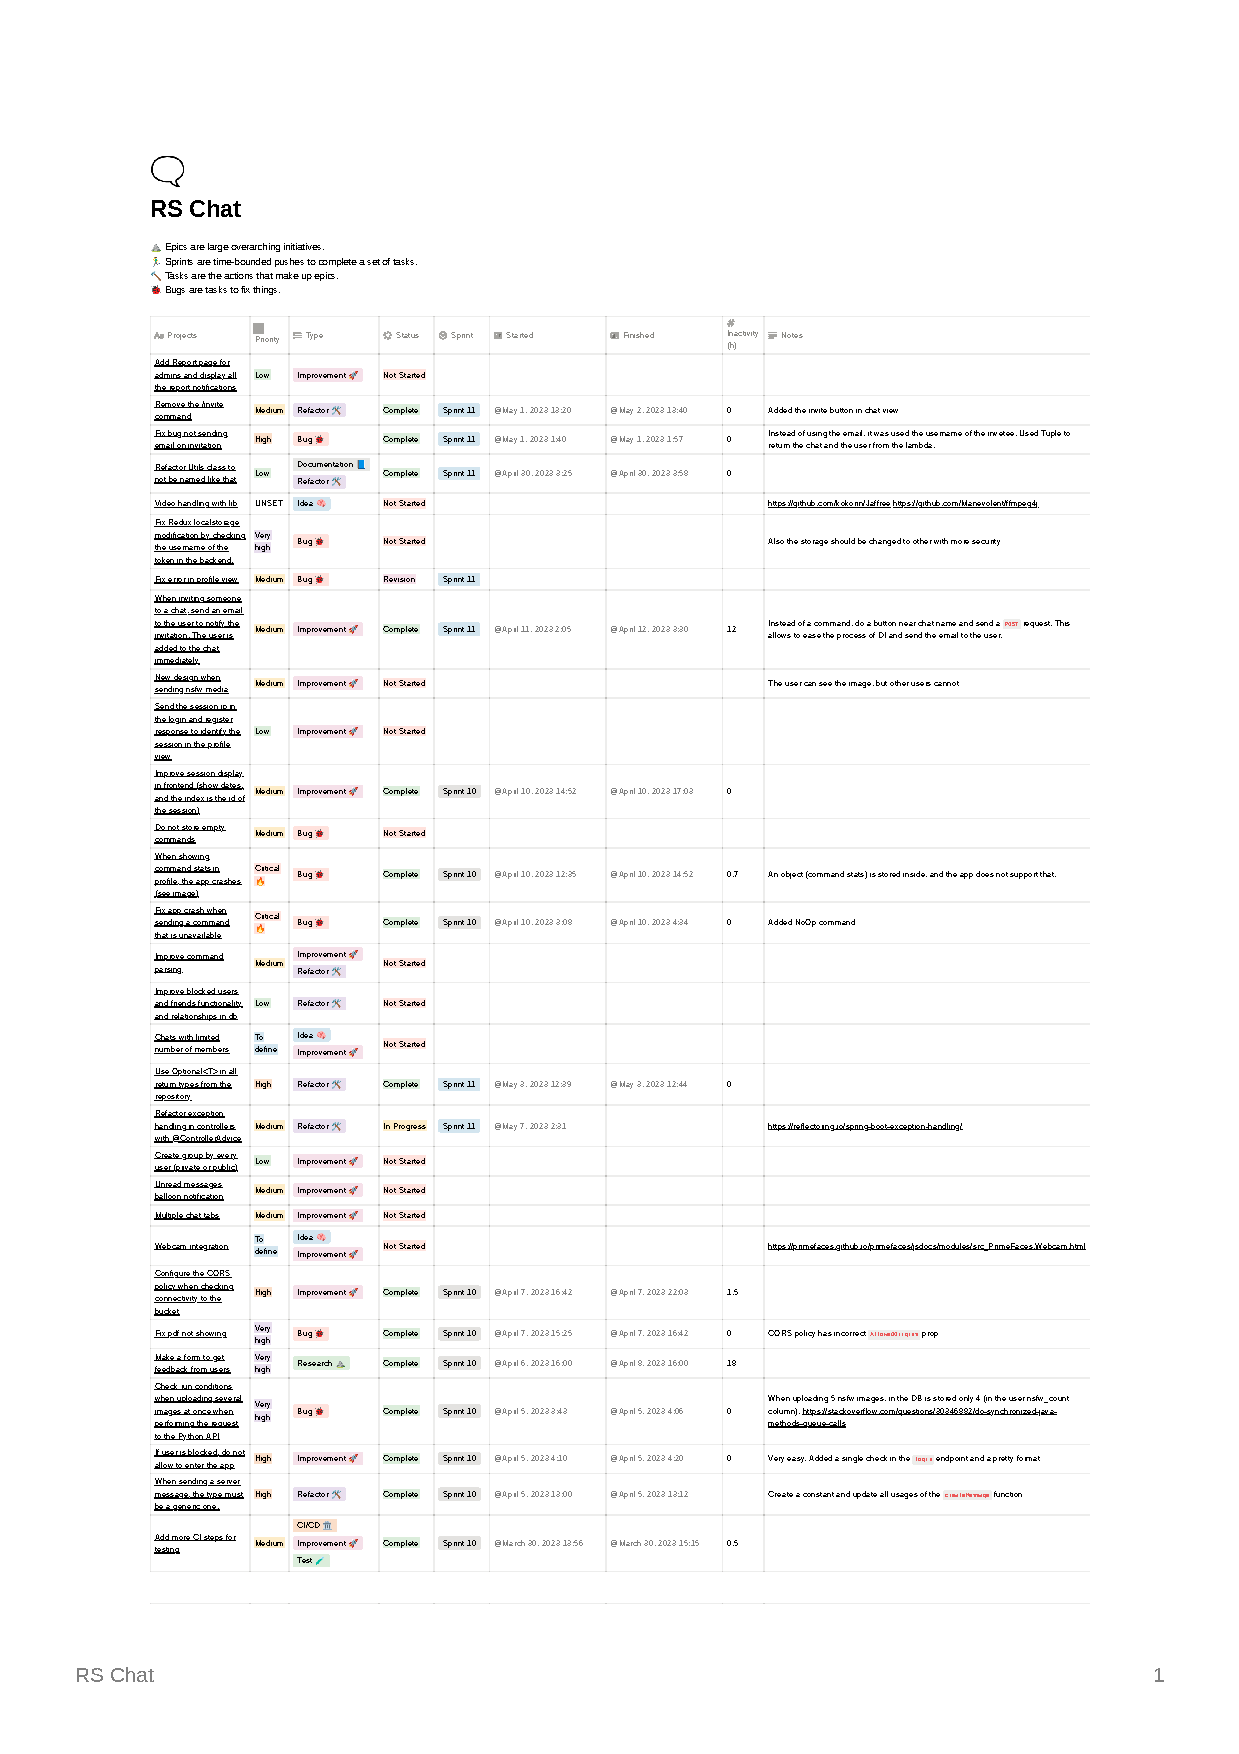
\includepdf[pages=-]{anexos/TareasNotion.pdf}
